\documentclass{standalone}
\usepackage{tikz}

\begin{document}

\tikzset{every picture/.style={line width=0.75pt}} %set default line width to 0.75pt

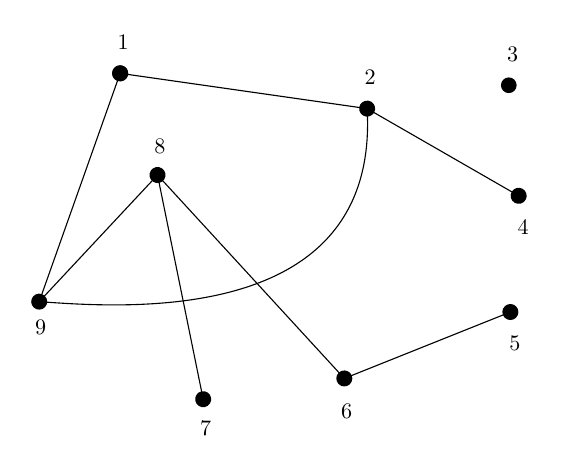
\begin{tikzpicture}[x=0.75pt,y=0.75pt,yscale=-1,xscale=1]
%uncomment if require: \path (0,462); %set diagram left start at 0, and has height of 462

%Straight Lines
\draw    (214.5,148) -- (175.5,258) ;
\draw [shift={(175.5,258)}, rotate = 109.52] [color={rgb, 255:red, 0; green, 0; blue, 0 }  ][fill={rgb, 255:red, 0; green, 0; blue, 0 }  ][line width=0.75]      (0, 0) circle [x radius= 3.35, y radius= 3.35]   ;
\draw [shift={(214.5,148)}, rotate = 109.52] [color={rgb, 255:red, 0; green, 0; blue, 0 }  ][fill={rgb, 255:red, 0; green, 0; blue, 0 }  ][line width=0.75]      (0, 0) circle [x radius= 3.35, y radius= 3.35]   ;
%Straight Lines
\draw    (214.5,148) -- (333.5,165) ;
\draw [shift={(333.5,165)}, rotate = 8.13] [color={rgb, 255:red, 0; green, 0; blue, 0 }  ][fill={rgb, 255:red, 0; green, 0; blue, 0 }  ][line width=0.75]      (0, 0) circle [x radius= 3.35, y radius= 3.35]   ;
\draw [shift={(214.5,148)}, rotate = 8.13] [color={rgb, 255:red, 0; green, 0; blue, 0 }  ][fill={rgb, 255:red, 0; green, 0; blue, 0 }  ][line width=0.75]      (0, 0) circle [x radius= 3.35, y radius= 3.35]   ;
%Straight Lines
\draw    (333.5,165) -- (406.5,207) ;
\draw [shift={(406.5,207)}, rotate = 29.91] [color={rgb, 255:red, 0; green, 0; blue, 0 }  ][fill={rgb, 255:red, 0; green, 0; blue, 0 }  ][line width=0.75]      (0, 0) circle [x radius= 3.35, y radius= 3.35]   ;

%Straight Lines
\draw    (175.5,258) -- (232.5,197) ;


%Straight Lines
\draw    (402.5,263) -- (322.5,295) ;
\draw [shift={(322.5,295)}, rotate = 158.2] [color={rgb, 255:red, 0; green, 0; blue, 0 }  ][fill={rgb, 255:red, 0; green, 0; blue, 0 }  ][line width=0.75]      (0, 0) circle [x radius= 3.35, y radius= 3.35]   ;
\draw [shift={(402.5,263)}, rotate = 158.2] [color={rgb, 255:red, 0; green, 0; blue, 0 }  ][fill={rgb, 255:red, 0; green, 0; blue, 0 }  ][line width=0.75]      (0, 0) circle [x radius= 3.35, y radius= 3.35]   ;
%Straight Lines
\draw    (254.5,305) -- (232.5,197) ;
\draw [shift={(232.5,197)}, rotate = 258.49] [color={rgb, 255:red, 0; green, 0; blue, 0 }  ][fill={rgb, 255:red, 0; green, 0; blue, 0 }  ][line width=0.75]      (0, 0) circle [x radius= 3.35, y radius= 3.35]   ;
\draw [shift={(254.5,305)}, rotate = 258.49] [color={rgb, 255:red, 0; green, 0; blue, 0 }  ][fill={rgb, 255:red, 0; green, 0; blue, 0 }  ][line width=0.75]      (0, 0) circle [x radius= 3.35, y radius= 3.35]   ;
%Straight Lines
\draw    (322.5,295) -- (232.5,197) ;


%Curve Lines
\draw    (175.5,258) .. controls (217,261) and (339.5,270) .. (333.5,165) ;


%Shape: Circle
\draw  [fill={rgb, 255:red, 0; green, 0; blue, 0 }  ,fill opacity=1 ] (398.25,153.75) .. controls (398.25,151.82) and (399.82,150.25) .. (401.75,150.25) .. controls (403.68,150.25) and (405.25,151.82) .. (405.25,153.75) .. controls (405.25,155.68) and (403.68,157.25) .. (401.75,157.25) .. controls (399.82,157.25) and (398.25,155.68) .. (398.25,153.75) -- cycle ;

% Text Node
\draw (216,133) node [scale=0.8]  {$1$};
% Text Node
\draw (335,150) node [scale=0.8]  {$2$};
% Text Node
\draw (403.67,139) node [scale=0.8]  {$3$};
% Text Node
\draw (408.67,222) node [scale=0.8]  {$4$};
% Text Node
\draw (404.67,278) node [scale=0.8]  {$5$};
% Text Node
\draw (323.67,311) node [scale=0.8]  {$6$};
% Text Node
\draw (255.67,319) node [scale=0.8]  {$7$};
% Text Node
\draw (176.17,270.5) node [scale=0.8]  {$9$};
% Text Node
\draw (233.67,183) node [scale=0.8]  {$8$};


\end{tikzpicture}

\end{document}
